\Section{Experimental Setup}
\label{ch:experiment}

In this chapter the experimental context of this thesis will be discussed. 

\Subsection{The Large Hadron Collider}
\label{sec:theory}

The Large Hadron Collider (LHC) is currently the most powerful particle accelerator in the world. Hosted at CERN in Geneva at the Swiss-French border and first put into operation on $\text{10}^\text{th}$ September 2008, the LHC is designed for proton and heavy lead ion collisions. The machine has gone through several upgrades between the consecutive data-taking phases (Runs) called Long Shutdowns (LS). During these the proton beam energy has been gradually increased from \SI{3.5}{\tera\electronvolt} to a recently (on the $\text{5}^{\text{th}}$ July, 2022) achieved energy of \SI{6.8}{\tera\electronvolt} \cite{Alici:2773265} resulting in a total centre-of-mass (CM) proton-proton collision energy of $\sqrt{s} = \SI{13.6}{\tera\electronvolt}$. Similarly, the beam intensity has seen an increase from $1.1 \times 10^{11}$ protons per bunch (ppb) and \textasciitilde200 bunches to a projected \textasciitilde$1.8 \times 10^{11}$ ppb and \textasciitilde2500 bunches \cite{Fartoukh:2790409, Karastathis:2750302}. With a theoretical maximum CM energy of $\sqrt{s} = \SI{14}{\tera\electronvolt}$ and instantaneous luminosity of $L = \SI{10d34}{\centi\meter^{-2}\second^{-1}}$ it holds the record in these measures among concurring experiments.

As a result of consecutive accelerator upgrades, the collider complex has an impressive and complex pre-accelerator structure as shown in fig. \ref{fig:lhcstructure}. Consequently, the proton bunches first go through multiple preparation steps before they get injected into the \SI{27}{\kilo\meter} tunnel of the LHC where the four main experiments (ALICE, ATLAS, CMS and LHCb) and their interaction points are located. 

\begin{figure}[h!]
	\centering
	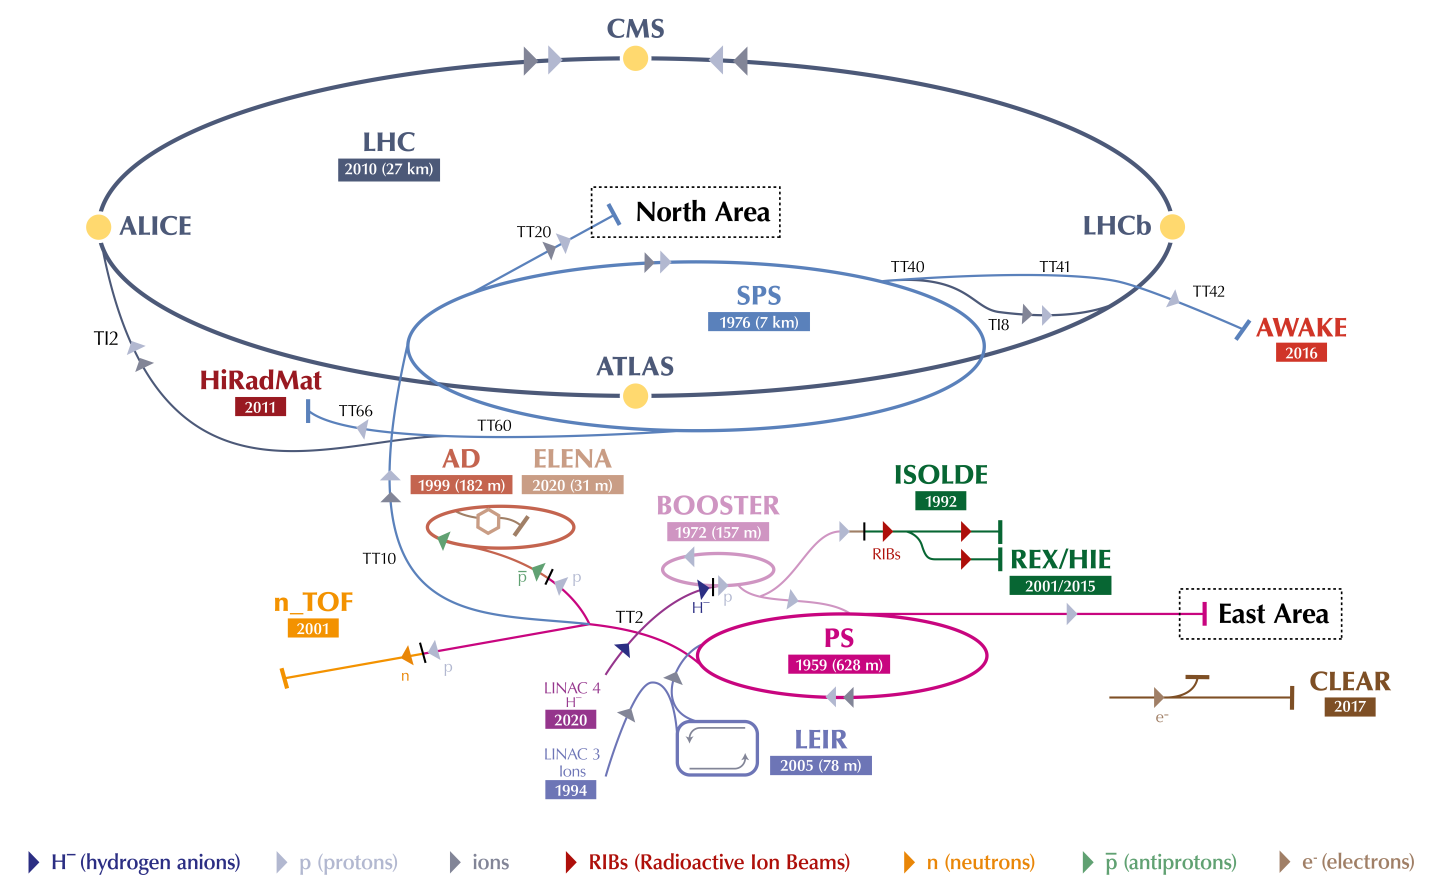
\includegraphics[width=0.8\linewidth]{figures/experiment/CCC-v2019-final-white_cut}
	\caption{The accelerator complex of the LHC, their corresponding construction years and circumferences. Individual stages are shown in different colours, the particle types they accelerate are indicated as arrows. Note that the pre-acceleators do not serve the LHC ring exclusively and the diverging paths lead to other independent experiments. Old tunnels of previous experiments serve as pre-accelerators now in the LHC injection chain. \cite{Mobs:2684277}}
	\label{fig:lhcstructure}
\end{figure}

The four main stages of pre-acceleration for protons are listed in tab. \ref{tab:preaccelerators} below. As proton source, hydrogen is used. The protons are first accelerated in the form of H$^-$ ions through the 86 metre long tunnel of the recently (2020) constructed Linear Accelerator 4 (Linac4). Stripped of their pair of electrons, the protons enter the Proton Synchrotron Booster (PSB) where they reach up to \SI{2}{\giga\electronvolt}. In the next step of the injection chain, they enter the Proton Synchrotron (PS), historically the first synchrotron at CERN serving exclusively as a pre-accelerator now. Travelling through the 628 metres long ring and accelerated to 26 GeV, the particles are injected into the Super Proton Synchrotron (SPS), where they are awaiting injection into the LHC once they reach 450 GeV.

%https://home.cern/science/accelerators/linear-accelerator-4
%https://home.cern/science/accelerators/proton-synchrotron-booster
%https://home.cern/science/accelerators/proton-synchrotron
%https://home.cern/science/accelerators/super-proton-synchrotron
%https://home.cern/science/accelerators/large-hadron-collider

\begin{table}[h!]
	\centering
	\begin{tabular}{c|c}
		Accelerator & Peak Energy \\
		\hline
		\hline
		Linear accelerator 4 (Linac4) & 160 MeV \\
		\hline
		Proton Synchrotron Booster (PSB) & 2 GeV \\
		\hline
		Proton Synchrotron (PS) & 26 GeV \\
		\hline
		Super Proton Synchrotron (SPS) & 450 GeV \\
		\hline
		Large Hadron Collider (LHC) & 7 TeV \\
	\end{tabular}
	\caption{The acceleration chain the protons undergo to reach their theoretical maximum energy of 7 TeV.}
	\label{tab:preaccelerators}
\end{table}

In the LHC the beams are circulating in opposing directions. They are kept on a circular trajectory using superconducting NbTi magnets operating at \SI{1.9}{\kelvin} thanks to the superfluid helium bath at about \SI{0.13}{\mega\pascal} \cite{Bruning:782076}. In the tunnel itself there are eight interaction points (IP). ATLAS, ALICE, CMS and LHCb are located at IP1, IP2, IP5 and IP8, respectively. IP3 and IP7 are where the momentum and betatron collimators are located ensuring beam quality; the radiofrequency (RF) cavities are at IP4 increasing the bunch energy to 7 TeV. The beam dump is at IP6 where old bunches are deflected by the fast-pulsing "kicker" magnets and directed towards the carbon absorber at the end of their lifetime. \cite{Evans_2008}

\begin{figure}[h!]
	\centering
	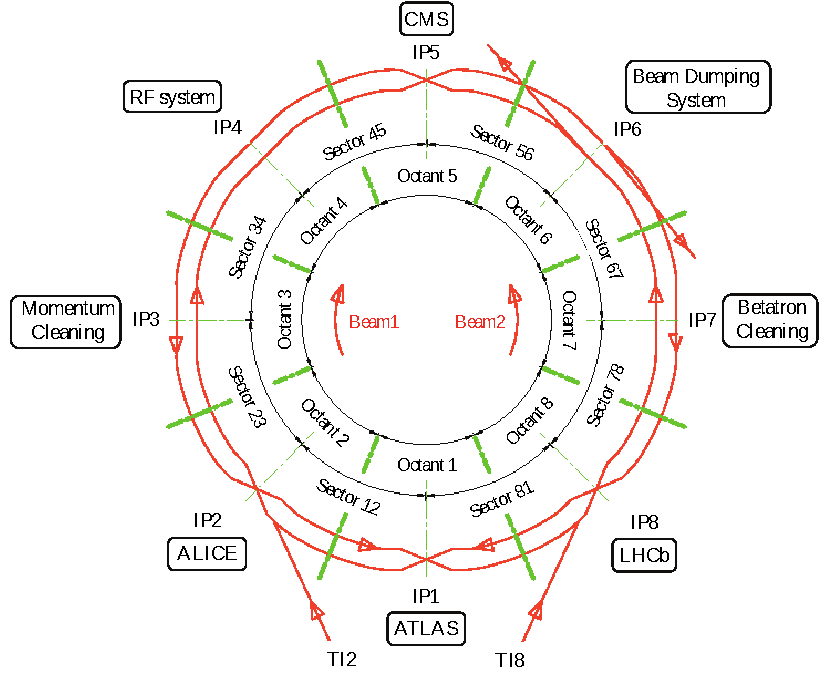
\includegraphics[width=0.6\linewidth]{figures/experiment/LHC_ring.pdf}
	\caption{The location of the interaction points, the experiments, and the beam adjustment systems. The LHC ring is also divided into further sectors and octants for each IP. \cite{Bracco:1174254}}
	\label{fig:LHC_ring}
\end{figure}

The four main detectors perform the particle collision measurements. LHCb specializes on flavour physics and measures b-quark decays focussing on the measurement and study of CP-violating processes. ALICE has been constructed to mainly study the quark-gluon plasma resulting from heavy ion collisions. ATLAS and CMS are sister experiments and are general purpose detectors. In the following, the latter will be described in detail only.

\Subsection{The Compact Muon Solenoid}

The Compact Muon Solenoid (CMS) detector is a 14 000 tonnes heavy detector measuring 28.7 metres in lenght and 15.9 metres in diameters. It has been built to be general purpose detector, featuring additional muon chambers at its most outer side allowing the precise measurement of muon momenta. The detector is built around a solenoid magnet, producing a magnetic field of $\SI{4}{\tesla}$. CMS has several subdetector components which surround the beampipe in a layered, onion-like structure. CMS has rotational symmetry around the beam pipe along which the z-axis is usually defined. The positions of each components and some of their most important technical details are shown in fig. \ref{fig:cms_view}.

\begin{figure}[h!]
	\centering
	\includegraphics[width=0.8\linewidth]{figures/experiment/cms_160312_02.pdf}
	\caption{The inner structure of the CMS detector. Note the layered structure and rotational symmetry of the detector. Each layer performs an individual step in particle identification. \cite{Sakuma:2665537}}
	\label{fig:cms_view}
\end{figure}

The coordinate system has its origin at the interaction point, is right-handed, with the $z$-axis pointing towards the anti-clockwise beam direction. Hence, the $xy$ plane lies orthogonal to the beam pipe. Instead of the polar angle directly the pseudorapidity 

\begin{equation*}
	\eta = -\ln\tan\frac{\theta}{2}
\end{equation*}

is used, as it is an Lorentz-invariant quantity along the beam. $\eta = \pm\infty$ hence corresponds to the beampipe and $\eta = 0$ defines the $xy$ (transversal) plane. Using the pseudorapidity, the differences in the $\eta-\phi$ plane can be given by

\begin{equation*}
	\Delta R = \sqrt{\left(\Delta\eta\right)^2 + \left(\Delta\phi\right)^2}
\end{equation*}

With that, particle kinematics can be described in terms of their energy $E$, the transversal momentum $p_T$, $\eta$, $\phi$ and their mass $m$. In some cases, instead of the pseudorapidity, the rapidity

\begin{equation*}
	y = \frac{1}{2}\ln\frac{E+p_z}{E-p_z}
\end{equation*}

is used.

In the following, the main subdetector components, their location and role focussing on high $p_T$ events will be briefly described.

\Subsubsection{Silicon Tracking}

CMS has an all-silicon tracking system, which lies at the core of the detector close to the beam pipe. As the name suggests, the tracking system enables the reconstruction of the trajectories of the child particles passing through the detector. It thus plays a crucial role in particle identification as the charge of particles can be inferred from the track signature (or the lack thereof); apart from that, it also enables secondary vertex reconstruction of short-living secondary particles. Particles passing through the silicon ionize the tracker, producing a signal.

Having a length of 5.4 metres and a diameter of 2.4 metres it covers the pseudorapidity range $|\eta|<2.5$, the best tracking efficiency being in the barrel region $|\eta| < 0.9$ \cite{Veszpremi_2014}. Closest to the interaction point lies the pixel silicon tracker. Made-up of four cylindrical layers at $\SI{3}{\centi\meter}$, $\SI{7}{\centi\meter}$, $\SI{11}{\centi\meter}$ and $\SI{16}{\centi\meter}$ from the beam pipe at disks at the end, it is segmented into 124 million pixels of $\SI{100}{\micro\meter} \times \SI{150}{\micro\meter}$ and kept at $\SI{-20}{\degreeCelsius}$ during operation.

Outside of the silicon pixel detector lie the silicon strip detectors, which is divided into four parts: the inner barrel par (TIB), the inner disk part (TID), the outer barrel (TOB) and the outer endcap part (TEC). This part of the tracker contains about 10 million strip components. The complete layout of the strip detectors is shown in fig. \ref{fig:strip_tracker}.

\begin{figure}[h!]
	\centering
	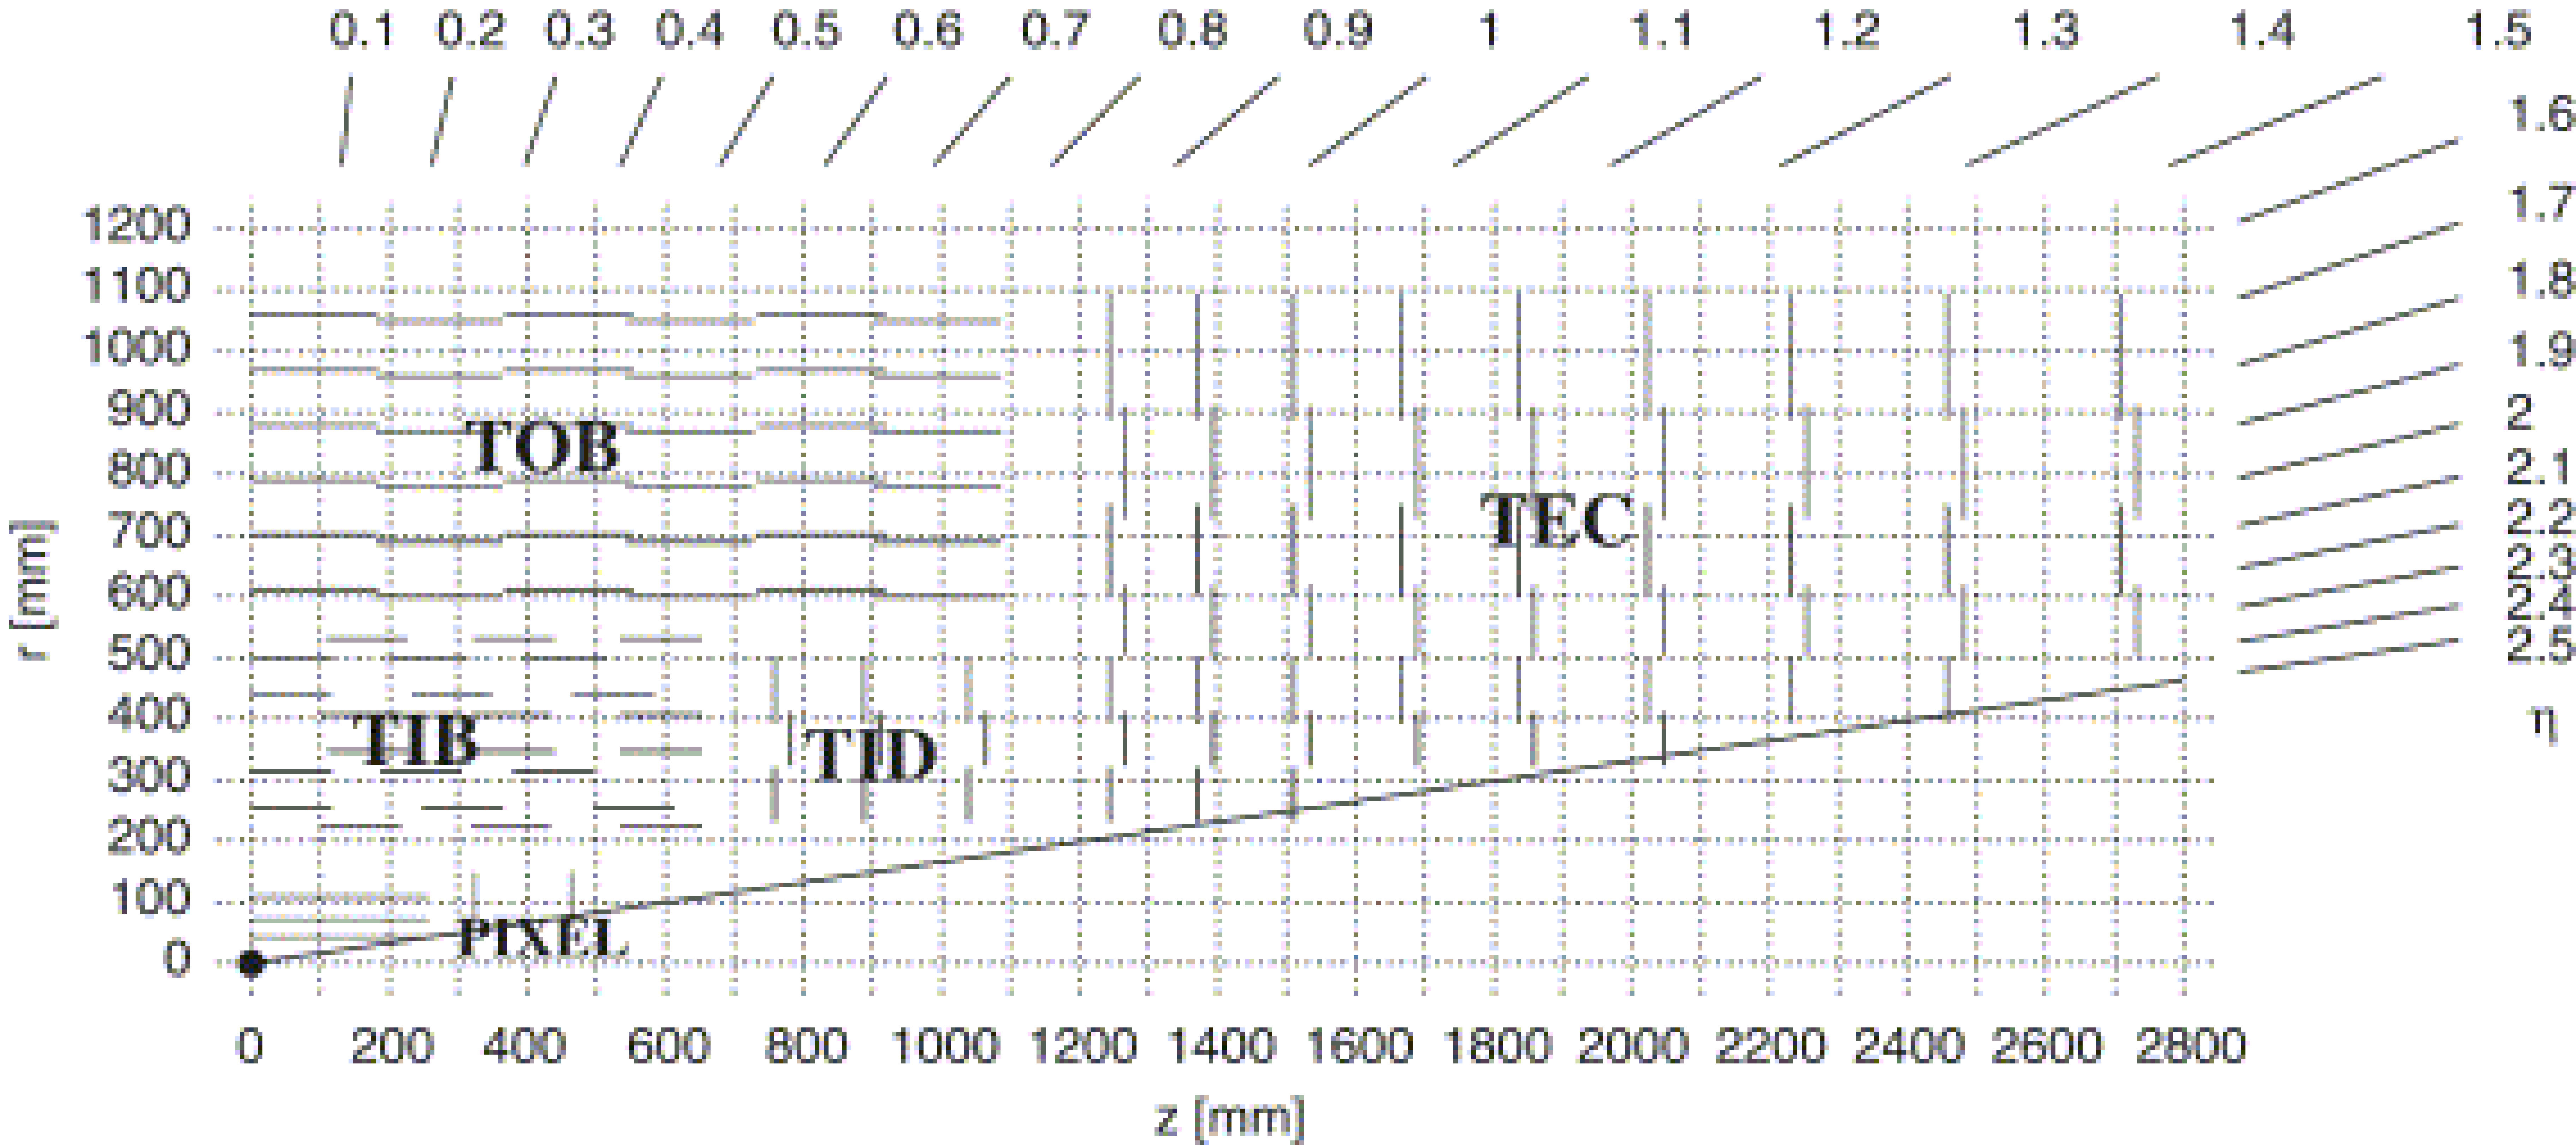
\includegraphics[width=0.8\linewidth]{figures/experiment/StripTracker}
	\caption{View of one quarter of the silicon strip detectors in the $r-z$ plane, indicating both the geometry and the pseudorapidity range of the individual parts. \cite{Azzurri:914891}}
	\label{fig:strip_tracker}
\end{figure}

\Subsubsection{Electromagnetic Calorimeter}

The CMS electromagnetic calorimeter (ECAL) measures the energy of electrons and photons by absorbing them completely and measuring the induced particle shower during the process. It lies outside of the tracking system and consists of highly transparent and scintillating lead tungstate (PbWO$_4$) crystals. The ECAL consists of two components as well, and central barrel (EB) covering the region up to $|\eta| = 1.48$ and an endcap region (EE) extending this coverage to pseudorapidities of $|\eta| = 3.0$ \cite{Biino_2015}. The EB has 61 200 crystals, which are formed into modules weighing around $\SI{3}{\tonne}$ and containing 1700 crystals, which are $\SI{23}{\centi\meter}$ (or $25.8 X_0$ in terms of radiation length $X_0$) in length. The EE at the end of the barrel modules have almost 15 000 more crystals; the total volume of the crystals is $\SI{11}{\cubic\meter}$ with a weight of $\SI{92}{\tonne}$. The layout of the calorimeter structure is shown in fig. \ref{fig:ecal}.

\begin{figure}[h!]
	\centering
	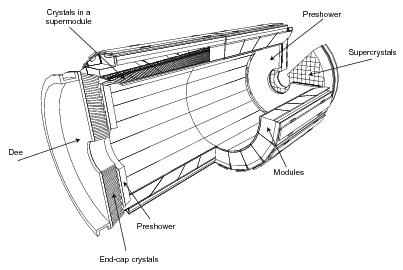
\includegraphics[width=0.6\linewidth]{figures/experiment/ecal.png}
	\caption{Schematic view of the CMS barrel and endcap calorimeters. Note the coverage around the tracker (not shown explicitly) and the preshower module, responsible for better seperation of photon hits in the endcap region. \cite{Chatrchyan:1554142}}
	\label{fig:ecal}
\end{figure}

The energy resolution of the barrel calorimeters has tree terms: a stochastic, a noise and a constant term and was measured to be \cite{Chatrchyan:1554142}

\begin{equation*}
	\frac{\sigma_E}{E} = \underbrace{\frac{2.8\%}{\sqrt{E\left[GeV\right]}}}_\text{stochastic} \oplus \, \underbrace{\vphantom{\frac{2.8\%}{\sqrt{E\left[GeV\right]}}}\frac{12\%}{E\left[GeV\right]}}_\text{noise} \oplus \, \underbrace{\vphantom{\frac{2.8\%}{\sqrt{E\left[GeV\right]}}}0.3\%}_\text{constant}
\end{equation*}

%In the barrel region the crystals are equipped with avalanche photodiodes (APD) of $5 \times \SI{5}{\square\milli\meter}$ and they are insensitive to the $\SI{4}{\tesla}$ magnetic field in the detector.

\Subsubsection{Hadronic Calorimeter}

The CMS hadronic calorimeters (HCAL) is a sampling calorimeter. Similarly to the ECAL, its purpose is to measure the energy of hadrons by measuring the induced avalanche of secondary particles upon passing through the detector as they are not directly stopped in the ECAL. In the $|\eta|<3$ region it consists of a brass scintillator calorimeter; in the forward region $3<|\eta|<5$ in has a iron quartz-fiber calorimeter \cite{canko_ak_2009}. It is organized into barrel (HB), outer barrel (HO), endcap (HE) and forward (HF) regions. The layout and the positioning of the respective components are shown in fig. \ref{fig:hcal}. Combined with the ECAL, the HCAL measures jets with a resolution of \cite{Lopez}

\begin{equation*}
	\frac{\sigma_E}{E} = \frac{100\%}{\sqrt{E\left[GeV\right]}} \oplus 5\%
\end{equation*}

\begin{figure}[h!]
	\centering
	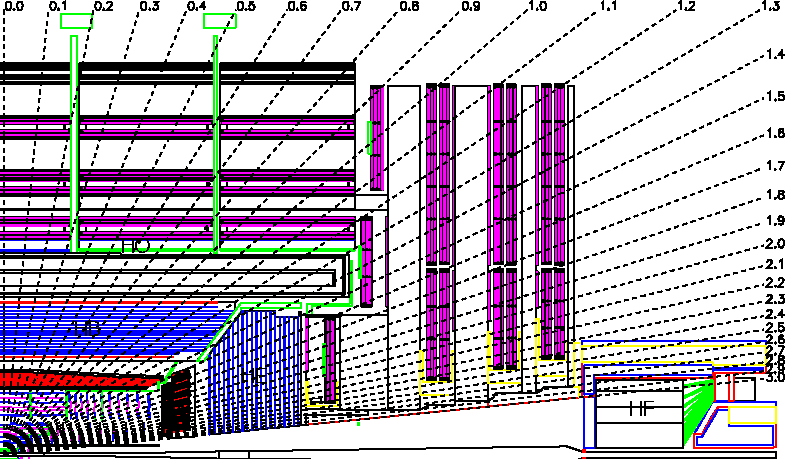
\includegraphics[width=0.8\linewidth]{figures/experiment/hcal.pdf}
	\caption{The CMS HCAL module setup. Note that the outer calorimeter lies outside of the solenoid (the white rectangle between HB and HO). \cite{Chatrchyan:1129810}}
	\label{fig:hcal}
\end{figure}

\Subsubsection{Superconducting Solenoid Magnet and the Return Yokes}

A core component of the detector is the solenoid magnet itself. Weighing $\SI{12000}{\tonne}$ and cooled down to $\SI{-268.5}{\degreeCelsius}$ it can produce a magnetic field of $\SI{4}{\tesla}$ ($\SI{3.8}{\tesla}$ during the runs) and is the largest solenoid in the world. The solenoid magnet and the return yokes play a crucial role in particle identification and muon measurement. These high magnetic fields are achieved using NbTi coils and a current of $\SI{18160}{\ampere}$. Outside of the solenoid magnet itself lie the muon chambers and the five return yokes, which are constructed from steel. The field strength thanks to the yokes there is around $\SI{2}{\tesla}$.

\Subsubsection{Muon Chambers}

In the outermost layers of the detector, the muon chambers can be found. CMS specializes in muon measurements and these chambers are characteristic for the whole detector. As muons provide a clear signature (like in a $H \rightarrow ZZ \rightarrow \mu\mu\mu\mu$, often referred to as the "Golden Channel"), their reconstruction is highly motivated. Due to muons having several orders of magnitude higher mass compared to electrons, they can pass the ECAL and they are not stopped by it.  Hence, they do not deposit their complete energy there meaning they can escape all the inner detector components. For this reason, additional measurements on their momenta are needed.

The chambers have four subcomponents: the drift tubes (TB), the cathode strip chambers (CSCs), the resistive plate chambers (RPCs) and the gas electron multipliers (GEMs), all of which are gaseous detectors. In the region $|\eta|<1.2$ the four layers of drift tubes have been installed at a radius of approximately $\SI{4}{\meter}$, $\SI{4.9}{\meter}$, $\SI{5.9}{\meter}$ and $\SI{7}{\meter}$. The tubes consist of 250 chambers and looking from the transversal plane, they are grouped into 12 sectors, with each covering 30° azimuthal angle. These chambers are staggered in a way, such that a high $p_T$ muon produced a the sector boundary crosses at least 3 of the four layers. In the endcap region up to $|\eta| < 2.4$, the CSCs are deployed. The CSCs are used both in the endcap and the barrel region. The newly added GEMs have been installed in the region $1.6 < |\eta| < 2.2$ \cite{Colaleo:2021453}. The exact position of the components are shown in fig. \ref{fig:muonchambers}.

\begin{figure}[h!]
	\centering
	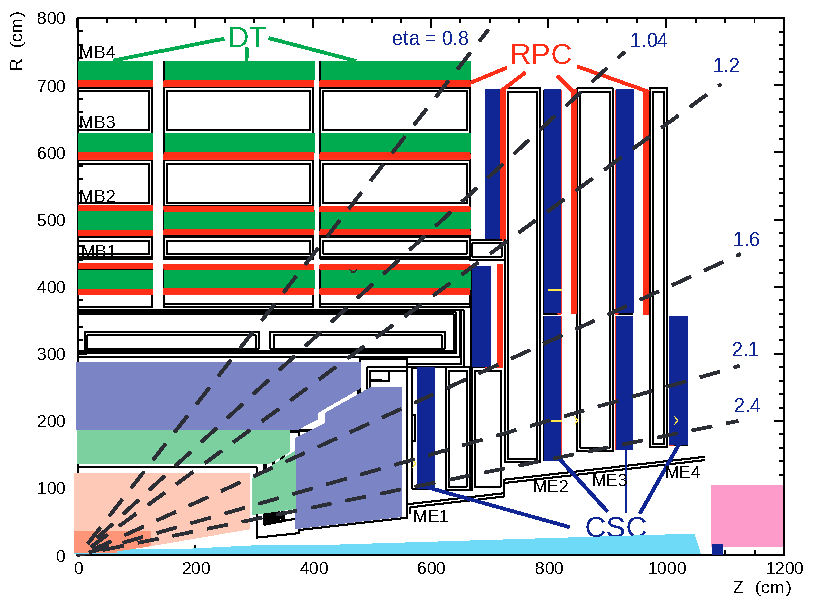
\includegraphics[width=0.8\linewidth]{figures/experiment/muonchambers.pdf}
	\caption{The location of the drift tubes (DT), the cathode strip chambers (CSCs) the resistive plate chambers (RPCs). The newly deployed GEMs are in the region $1.6 < |\eta| < 2.2$ (not shown here) \cite{Bayatian:922757}.}
	\label{fig:muonchambers}
\end{figure}

\Subsubsection{Trigger System}

With a collision frequency of $\SI{40}{\mega\hertz}$ with a new collision in every $\SI{25}{\nano\second}$ it is both impossible and unnecessary to record every event in the detector; impossible because the complete registration of this enormous data-flow is technologically infeasible and unnecessary as most of these events arise from soft collision processes. For this reason, a filtering (triggering) mechanism has been implemented in the detector.

The trigger system reduces the dataflow in two steps. The Level-1 (L1) trigger operates on a hardware level and reaches a decision in less than $\SI{1}{\micro\second}$. During the decision-making period, the high-resolution data is held the memory and increasingly complex algorithms are used to approach the quality of final reconstruction. These decisions involve information from the calorimeters and the muon systems and some correlation between them. It is based mostly on jet $E_T$ and $p_T$ thresholds and physics objects like photons, electrons and muons. The resulting data-stream from the L1 trigger is less than $\SI{100}{\kilo\hertz}$.

In the second step, the High-Level Triggers continue with the processing. They operate on a software level and have an output rate of $\SI{100}{\hertz}$ which can be stored offline for further analysis. Instead of fully reconstructing events from every detector component, they are first only partially reconstructed and eventually discarded as soon as possible \cite{Bayatian:922757}.

\Subsection{Physics Object Reconstruction}
\Subsubsection{Particle Flow}

Individual particles leave (up to the detector resolution) unique event signatures in each subdetector component, which is summarized in fig. \ref{fig:cms_slice}. In order to perform a complete physics analysis, these event signatures have to be assigned to physically interpretable objects in order to obtain the physical final state and kinematics such as energy, momenta and charge.

\begin{figure}[h!]
	\centering
	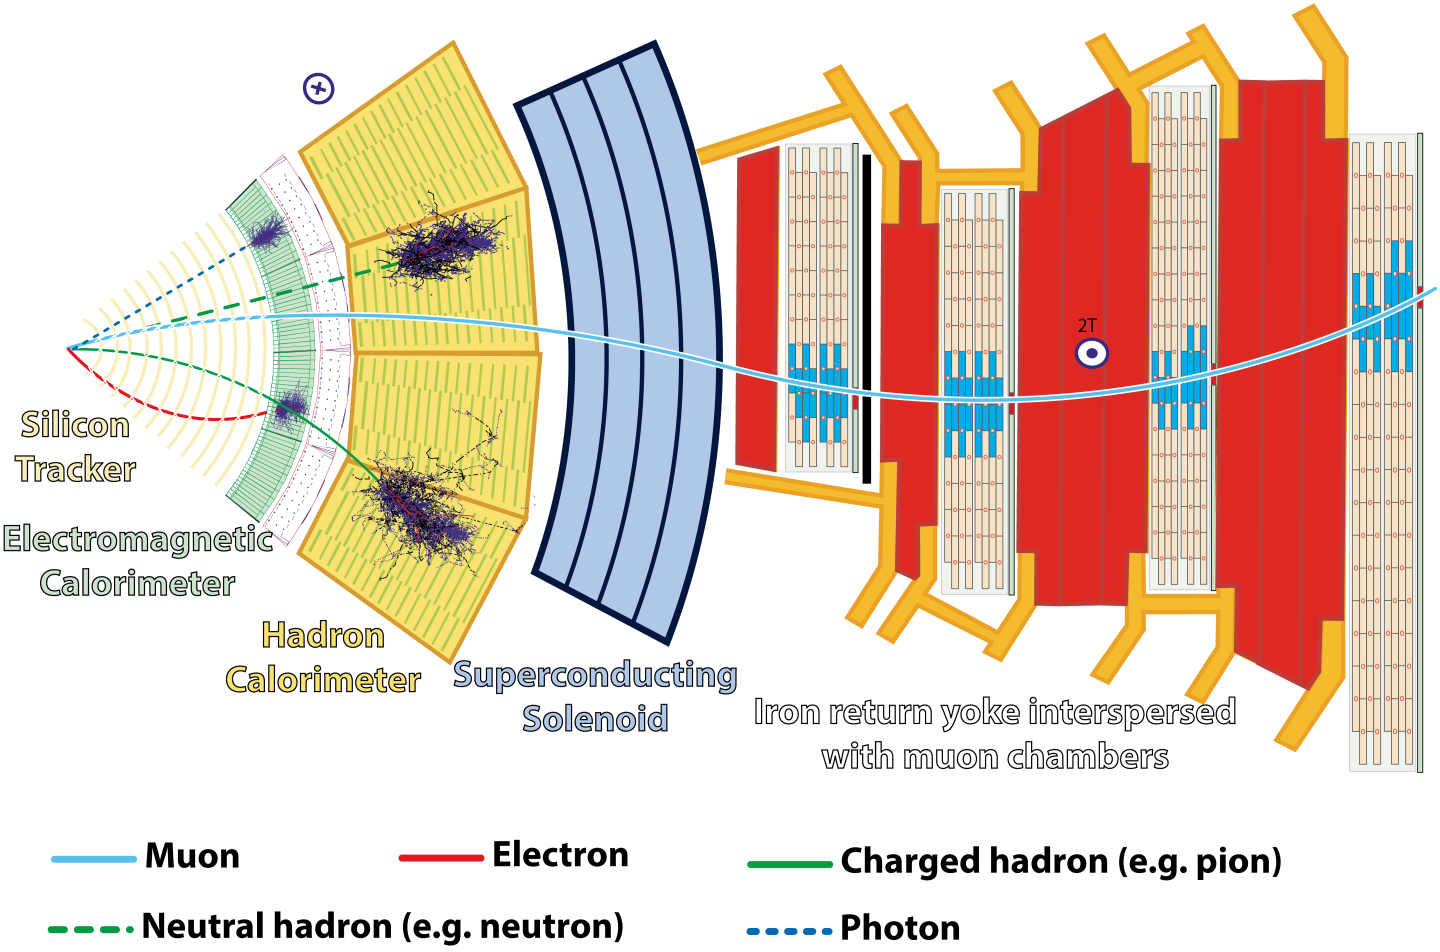
\includegraphics[width=0.8\linewidth]{figures/experiment/CMS_Slice}
	\caption{Transversal view of a slice of the CMS detector with several characteristic signatures drawn in different colours. Note that each detector slice functions as a filter for different particle kinds, i.e. the number of signatures decreases towards the outer layers. \cite{Barney:2120661}}
	\label{fig:cms_slice}
\end{figure}

The reconstruction algorithm used at the CMS experiment is Particle Flow (PF) \cite{Sirunyan_2017}. In order to obtain the physics objects, it first combines the particle tracker hits (both from the tracker and from the muon chambers) and clusters the energy deposits in the calorimeters. In order to keep the number of misreconstructed tracks minimal during track reconstruction several quality fit criteria are relaxed with each iteration. For the calorimeter clusters, an expectation-maximization algorithm based on a Gaussian-mixture model is used to reconstruct the clusters within the computed topological clusters around the pre-constructed cluster seeds.

Following that, the link algorithm is executed which connects the aforementioned PF elements from different subdetectors. At this point, it cannot be avoided that some particles are misidentified or wrongly reconstructed, especially in cases where a large missing transverse momentum $p^{miss}_T$ is present in the event. As such events (usually originating from misreconstructed high $p_T$ muons) may be wrongly selected by a large set of new physics searches, they undergo a post-processing algorithm in order to correct these effects.

Finally, the reconstructed particles are used to build the physics objects, namely jets, missing transverse momenta $p^{miss}_T$, muon, electrons and taus and other related quantities. Note that as a hadron collider, the exact centre-of-mass system is a priori unknown due to the interacting partons within the proton structure, hence the missing momenta can only be evaluated in the transversal plane.

\Subsubsection{Jet Clustering}

The hadronisation and fragmentation processes give rise to an avalanche of secondary particles in the detector called jets. Their reconstruction requires sophisticated tools to assign the detector hits to specific clusters. Such algorithms should ideally satisfy two requirements: they should be infrared and collinear safe, i.e. they should not be disturbed by soft emmisions (particles with low momenta) while collinear particles belonging to the same jet should be assigned correctly. CMS uses the anti-$k_T$ algorithm, a generalization of the $k_t$ and Cambridge/Aachen algorithm \cite{Cacciari_2008}. They are given by\footnote{Setting $p=0$ yields the Cambridge/Aachen algorithm, while $p=1$ one recovers the $k_t$ algorithm.}

\begin{equation*}
	\begin{aligned}
		d_{ij} &= \min\left(k^{2p}_{ti}, k^{2p}_{tj}\right)\frac{\Delta^2_{ij}}{R^2} \\
		d_{iB} &= k^{2p}_{ti}
	\end{aligned}
\end{equation*}

where $\Delta^2_{ij} = (y_i-y_j)^2 + (\phi_i - \phi_j)^2$ is the distance in the plane spanned by the rapidity $y$ and the azimuthal angle $\phi$ between particles $i$ and $j$, $R$ is a radius parameter, $k_{ti}$ is the transverse momentum of particle $i$ and $d_{iB}$ is the distance between the particle and the beam. Setting the parameter $p$ to $p=-1$ results in the both infrared, collinear safe and fast anti-$k_t$ algorithm.

Anti-$k_t$ accumulates soft particles which are in a radius $R$ of a hard particle if no other hard neighbours are present within $2R$  to the hard particle themselves in a perfectly conical jet. If there is another hard particle with $R < \Delta<2R$, then two not necessarily conical jets will be returned; for $\Delta<R$, both particles will form a single jet. From here one can see the stability of the algorithm with respect to soft emmisions while maintaining collinear safety.

One can differentiate two kinds of jets depeding on the radius $R$. $R=0.4$ or $R=0.8$ results in AK4 (resolved) or AK8 (boosted\footnote{or, in "CMS slang": fat}) jets, respectively. Nevertheless, the quark flavour which produces the jet cannot simply be obtained by jet clustering. Consequently, flavour identification (flavour tagging) has to be performed separately.

\Subsubsection{Flavour Tagging}

Assigning flavour to the jet-inducing quarks is possible through several heavy-flavour jet discriminating variables, which can be reconstructed by deep neural networks \cite{Sirunyan_2018}. Below a list and a description of some of these variables will be given.

For b quarks, the displacement of the secondary vertex due to the long enough lifetime of b hadrons which is at the order of $\SI{1.5}{\pico\second}$ (which corresponds to displacements of a few mm to $\SI{1}{\centi\meter}$) can be reconstructed. These displacements can be resolved with the tracker and can be characterized by the impact parameter (which is defined as the vector pointing from the primary vertex to the point of closest approach) of the child particles. Due to the heavier mass of the b and c quarks, the decay products have a larger transversal momentum with respect to the jet axis yielding larger impact parameter vectors compared to those of their light counterparts. In addition to that, in approximately 20\% and 10\% of the cases in the decay chain of b and c hadrons, respectively, a muon or an electron is present, which can be further used for heavy-flavour jet identification. The geometry of a general heavy decay is shown in fig. \ref{fig:pvsv}.

\begin{figure}[h!]
	\centering
	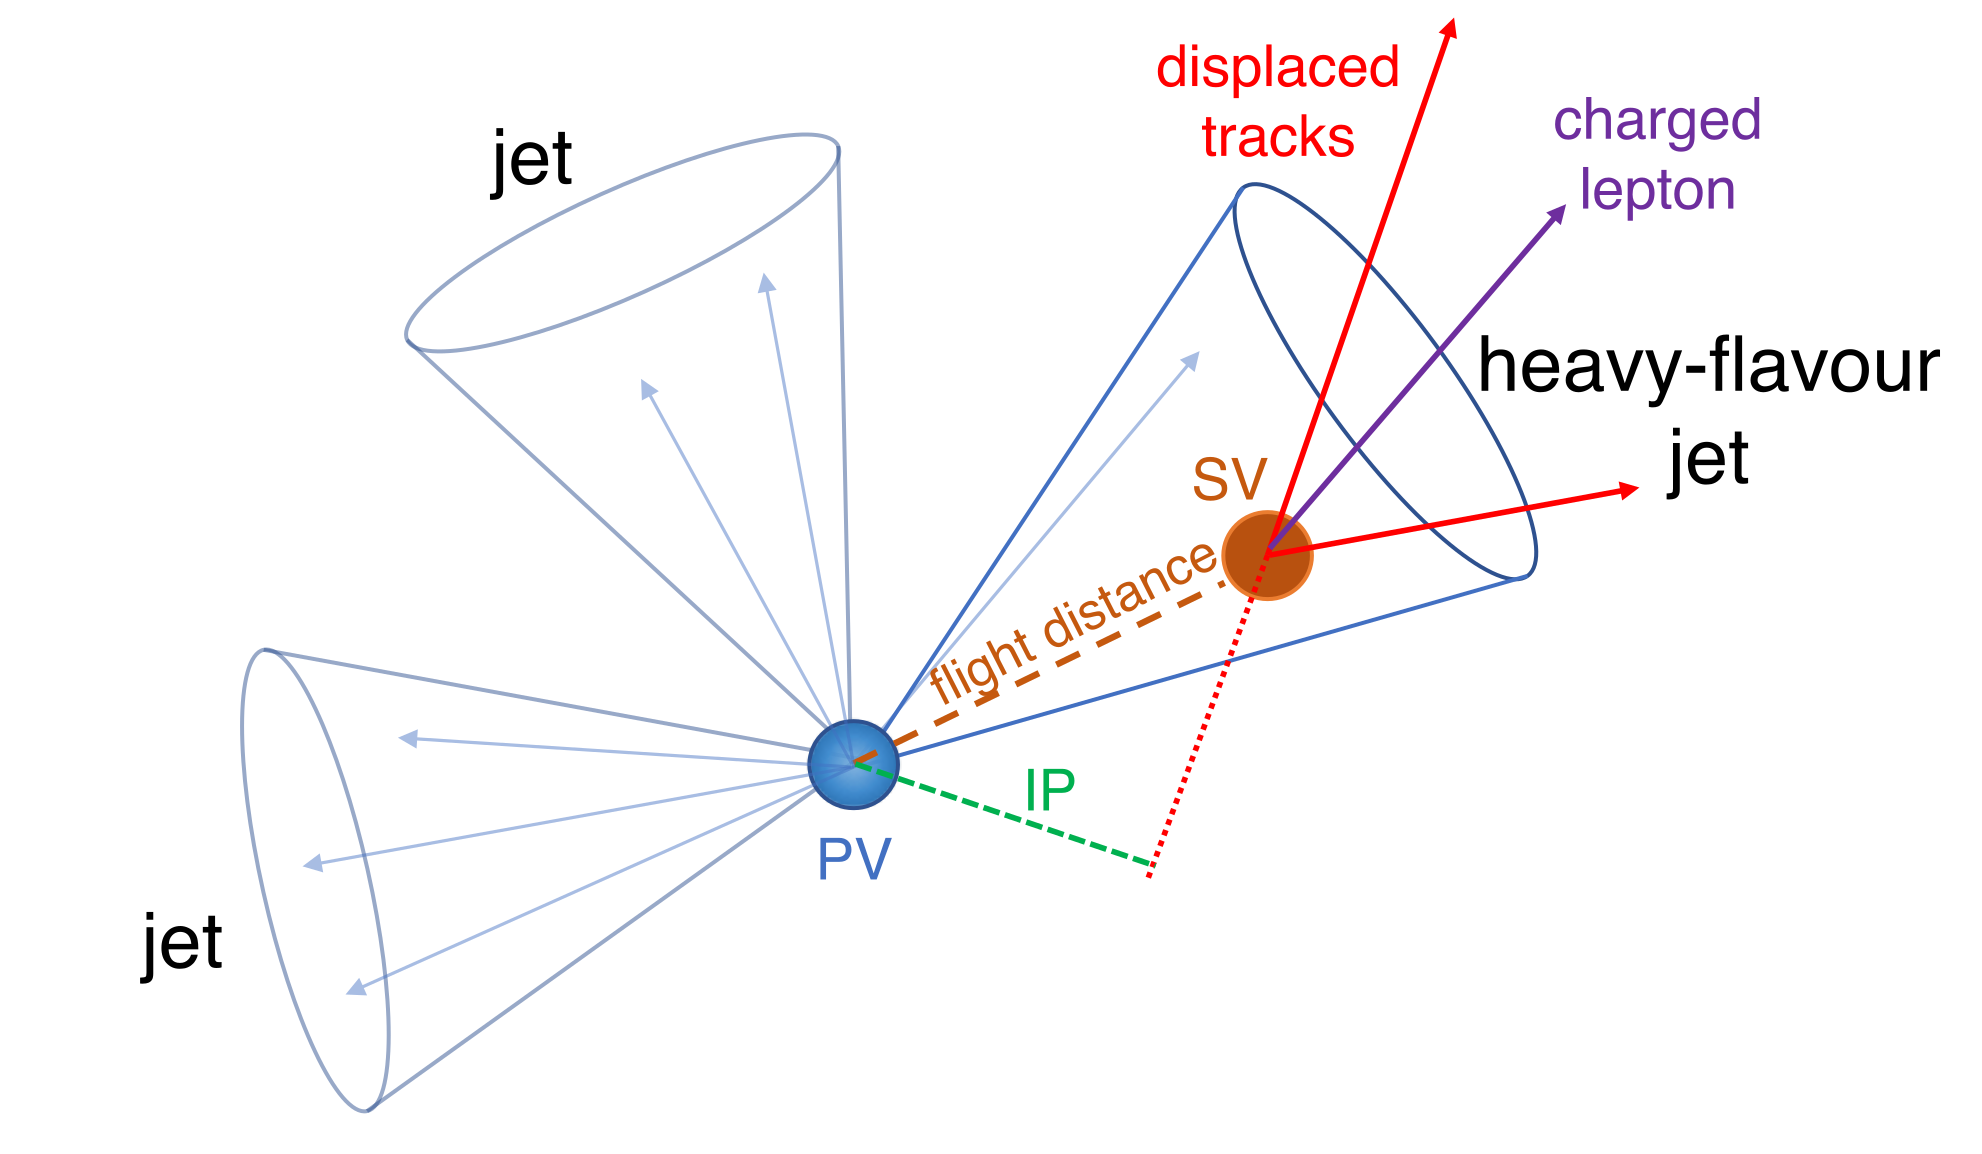
\includegraphics[width=0.6\linewidth]{figures/experiment/pvsv}
	\caption{Schematic view of the displacement of the secondary vertex with respect to the primary vertex with the definition of the impact parameter indicated. Note the possible appearence of a soft lepton (shown in purple) in the jet cone characteristic for heavy-flavour jets.}
	\label{fig:pvsv}
\end{figure}

\Subsubsection{Muons}

Since muons can leave signatures in both the tracker and the muon system, they are reconstructed and categorized depending on the muon signal quality and their physics properties. For the track reconstruction, the three categories in increasing quality are: \cite{Collaboration_2010}

\begin{itemize}
	\item[] \textit{Standalone-muon tracks} are constructed from the CSC, RPC and DT signatures using a Kalman-filter technique.
	\item[] \textit{Tracker muon tracks} are built "from the inside out" by loose matching tracker tracks (with $p_T > \SI{0.5}{\giga\electronvolt}$ and a total momentum of $p>\SI{2.5}{\giga\electronvolt}$) to DT and CSC segments. tracks automatically qualify if at least one muon segment matches the extrapolated track.
	\item[] \textit{Global muon tracks} are obtained "outside-in" by matching the standalone-muon tracks with the tracker tracks with the Kalman filter.
\end{itemize}

Note that these categories are not disjoint. Thanks to the high resolution and efficiency of muon track reconstruction, approximately 99\% of the muons are reconstructed as either as a tracker track muon, global muon track or both.

Following the categorization by the tracks, the muon IDs are assigned \cite{Sirunyan_2018_muons}. Using the variables from the track fit, the following identification types are assigned:

\begin{itemize}
	\item[] \textit{Loose muon ID} are for muons selected by the PF algorithm which is either a tracker or global muon. This selection ensures the identification of prompt muons originating from the primary vertex or from light and heavy flavour decays while minimizing the rate of charged hadrons misidentified as muons.
	\item[] \textit{Medium muons} are prompt muons and muons from heavy flavour decays which carry the loose ID with tracker track hits of more than 80\% of the inner tracker layers.
	\item[] \textit{Tight muon IDs} suppress hadronic punch-through and muons from decay in flight. They are both tracker and global muons with at least pixel hit and hits from at least six inner layer tracker hits, fulfilling additional event geometric criteria.
	\item[] \textit{Soft muons} are low $p_T$ muons with high purity tracker track of the same tracker requirements as tight muons.
	\item[] \textit{High momentum muon IDs} are for muons with $p_T > \SI{200}{\giga\electronvolt}$. They are both tracker and global muons with the same tracker hit and event geometric requirements as tight muons. In addition to that, they need at least one hit from the muon system for the global muon.
\end{itemize}